
\label{subsec:appdix_mechanism}
% \begin{figure}[h!]
%     \centering
%     \includegraphics[scale=0.21]{./images/layerwise_change_ratios_tau2.png}
%     \caption{Layer-wise parameter change ratios across models}
%     \label{fig:model_scaling}
% \end{figure}
% \begin{figure*}[h!]
%     \centering

%     \begin{subfigure}{\linewidth}
%         \centering
%         \includegraphics[scale=0.21]{./images/layerwise_change_ratios_tau2.png}
%         \caption{$\tau^2$ Bench}
%         \label{fig:model_scaling_a}
%     \end{subfigure}

%     \vspace{0.5em} % 调整上下间距，可选

%     \begin{subfigure}{\linewidth}
%         \centering
%         \includegraphics[scale=0.21]{./images/layerwise_change_ratios_alf.png}
%         \caption{ALFWorld}
%         \label{fig:model_scaling_b}
%     \end{subfigure}

%     \caption{Layer-wise parameter change ratios across models}
%     \label{fig:model_scaling}
% \end{figure*}
% \begin{figure*}[t]
%     \centering

%     \begin{subfigure}{0.48\textwidth}
%         \centering
%         \includegraphics[width=\linewidth]{./images/layerwise_change_ratios_tau2.pdf}
%         \caption{$\tau^2$ Bench}
%         \label{fig:model_scaling_a}
%     \end{subfigure}
%     \hfill
%     \begin{subfigure}{0.48\textwidth}
%         \centering
%         \includegraphics[width=\linewidth]{./images/layerwise_change_ratios_alf.pdf}
%         \caption{ALFWorld}
%         \label{fig:model_scaling_b}
%     \end{subfigure}

%     \caption{Layer-wise parameter change ratios across models}
%     \label{fig:mechanism}
% \end{figure*}

\begin{figure*}[h]
    \centering

    % --------- Top: Layer-wise ---------
    \begin{subfigure}{\textwidth}
        \centering
        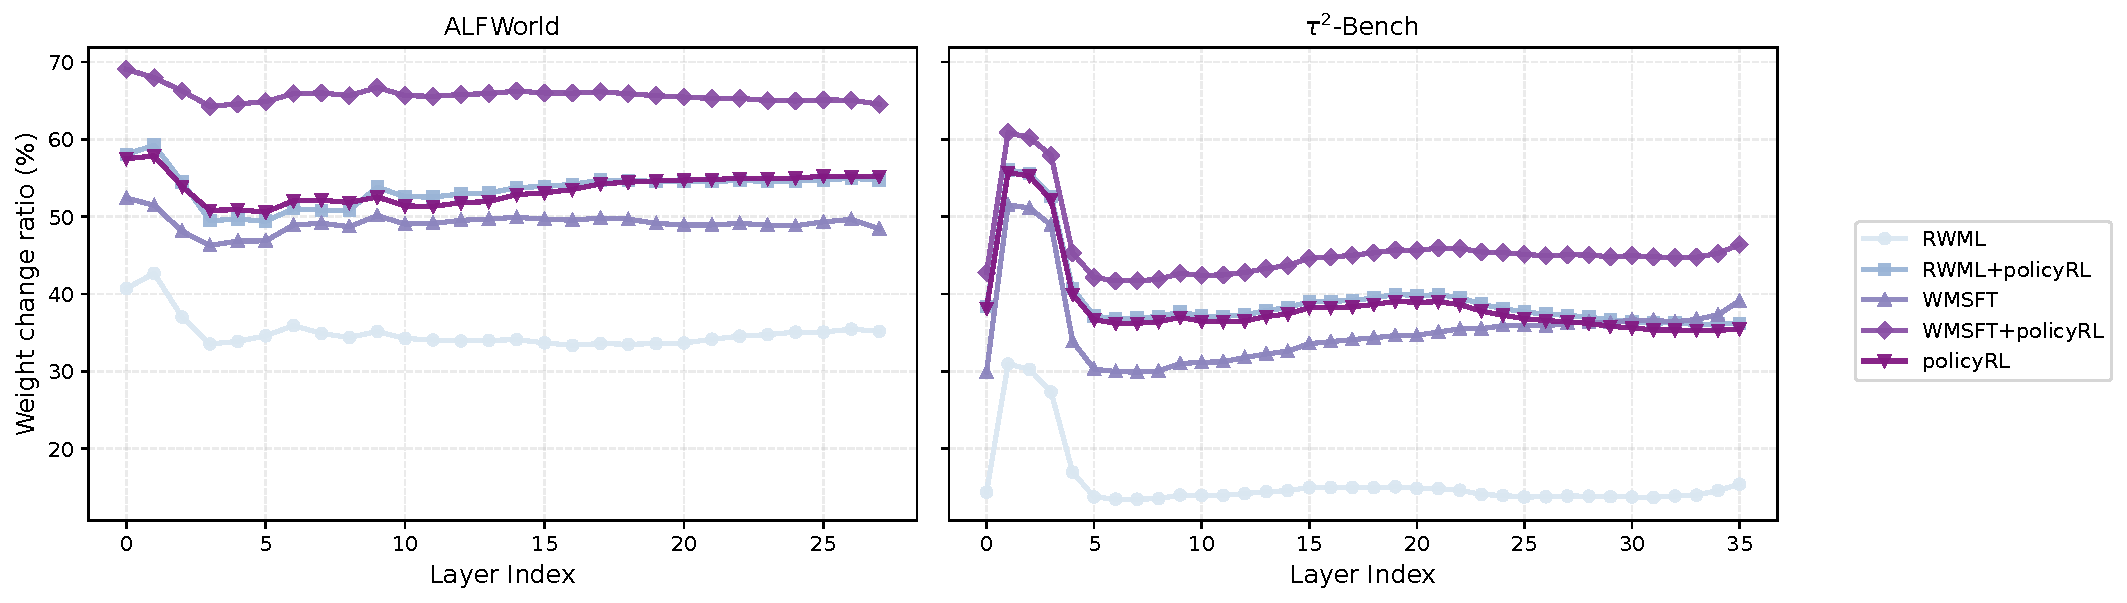
\includegraphics[width=\textwidth]{./images/layerwise_alf_tau_sharedlegend.pdf}
        \caption{Layer-wise parameter change ratios by transformer layer (ALFWorld and $\tau^2$-Bench).}
        \label{fig:mechanism_layerwise}
    \end{subfigure}

    \vspace{0.8em} % 调整上下两张图之间的距离（可改 0.4em ~ 1.2em）

    % --------- Bottom: Module-wise ---------
    \begin{subfigure}{\textwidth}
        \centering
        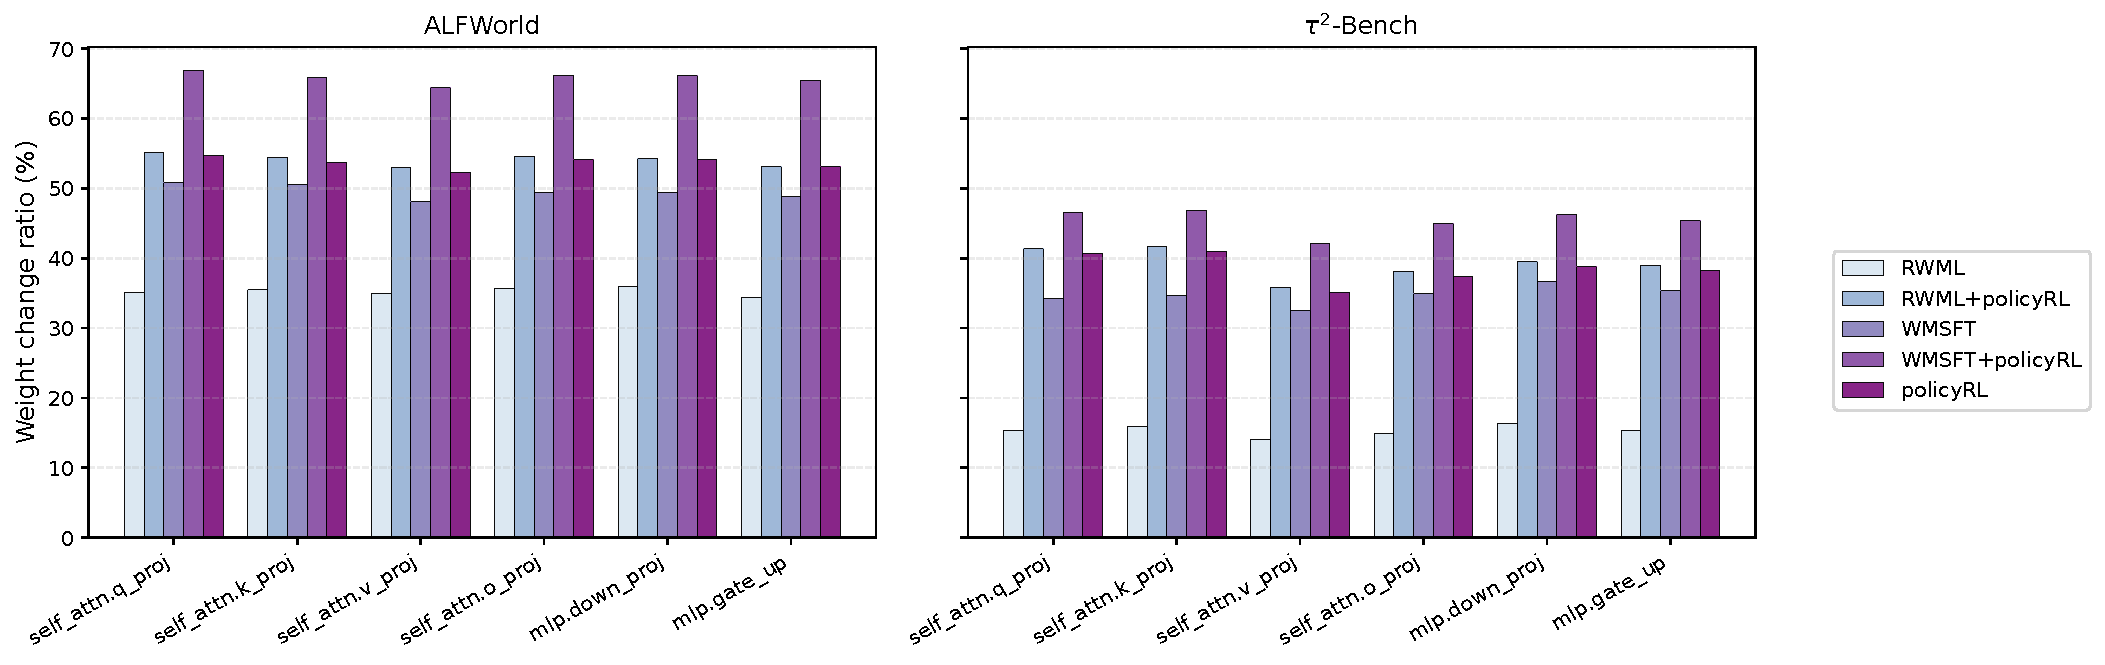
\includegraphics[width=\textwidth]{./images/modulewise_alf_tau_sharedlegend.pdf}
        \caption{Module-wise parameter change ratios aggregated across layers (attention Q/K/V/O and MLP projections).}
        \label{fig:mechanism_modulewise}
    \end{subfigure}

    \caption{
        Parameter change analysis across datasets and training variants.
        \textbf{Top:} layer-wise weight change ratios by transformer layer.
        \textbf{Bottom:} main module-wise change ratios aggregated across layers.
    }
    \label{fig:mechanism}
\end{figure*}


We report a fine-grained analysis of parameter updates at both the layer and module levels. Specifically, we compute the fraction of parameters exhibiting major changes within each transformer layer, with results summarized in \Cref{fig:mechanism_layerwise}. Across both benchmarks, we observe highly consistent trends throughout the network depth. Models trained with \wmrlshort{} display the lowest proportion of updated parameters, whereas \wmsftshort{} leads to noticeably broader parameter modifications. This pattern aligns with the forgetting behavior analyzed in \Cref{subsec:Forgetting}, where \wmrlshort{} models retain prior knowledge more effectively.

In addition, we compare the effects of policy RL when applied to different mid-trained initializations. Notably, the parameter change profiles of policy RL remain largely similar regardless of whether \wmrlshort{} is applied beforehand, and closely resemble those obtained when policy RL is performed directly on the base model. In contrast, initializing policy RL from a \wmsftshort{} model results in substantially elevated update ratios. These results indicate that \wmrlshort{} preserves a parameter configuration that is more amenable to subsequent policy optimization, reducing the extent of disruptive updates during post-training.

To further validate that this behavior is not an artifact of layer aggregation, we conduct a module-wise breakdown over attention projections (Q/K/V/O) and MLP projection parameters, as shown in \Cref{fig:mechanism_modulewise}. The observed trends closely mirror the layer-wise results, suggesting that the relative stability induced by \wmrlshort{} is consistent across different architectural components rather than being localized to specific modules.

Overall, these detailed analyses provide additional evidence that employing RL during both mid-training and post-training leads to more coherent and stable parameter update than the conventional SFT-then-RL pipeline. 

Finally, we emphasize that the analyses presented here are empirical and are intended to provide descriptive evidence rather than a complete mechanistic explanation. While the observed parameter update patterns offer insights into how \wmrlshort{} influences subsequent training dynamics, a more systematic understanding of RL-based training—particularly from the perspectives of optimization dynamics and mechanistic interpretability—remains an important direction for future work. We hope these findings motivate further investigation into the internal representations and learning trajectories induced by RL at different stages of model training.